\documentclass{xStandalone}

\begin{document}
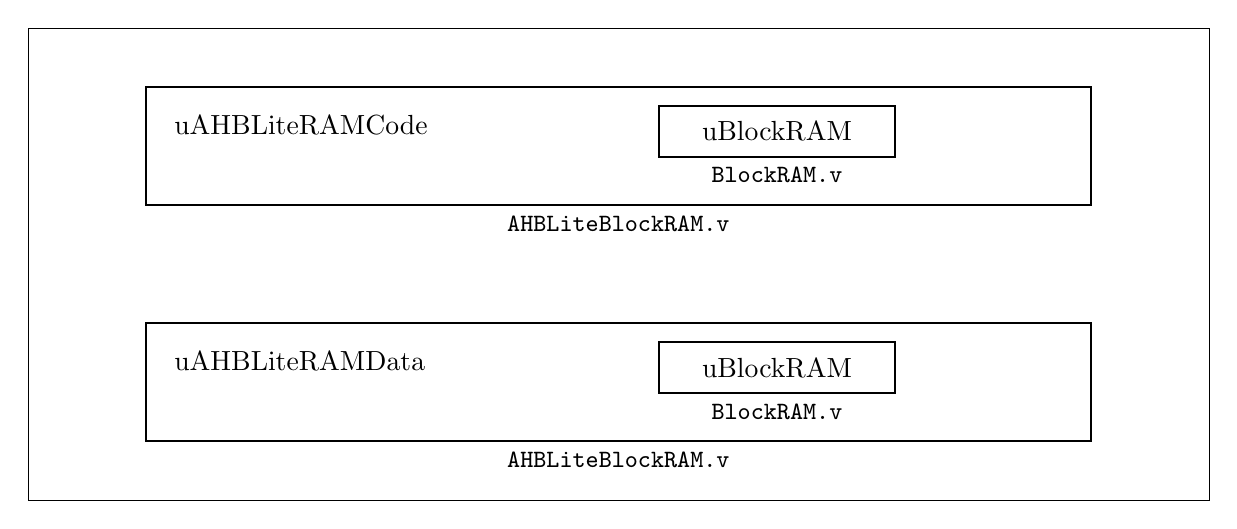
\begin{tikzpicture}
\tikzset{outerframe/.style=ultra thin,gray}

\tikzset{module/.style={
rectangle,draw,black,thick,
minimum width=3cm,
minimum height=0.65cm,
align=center}}

\tikzset{moduleBig/.style={
rectangle,draw,black,thick,
minimum width=12cm,
minimum height=1.5cm,
align=center}}

\draw[outerframe] 
(-7.5,-3) coordinate (A1) 
rectangle 
(+7.5,+3) coordinate (B2);

\path
(A1|-B2) coordinate (B1)
(A1-|B2) coordinate (A2);

\draw
(0,+1.5) 
node[moduleBig,name=uAHBCode] {}
(uAHBCode.north west) 
node[below right=0.25cm,black]
{uAHBLiteRAMCode}
(uAHBCode.south)
node[below,black] 
{\small\ttfamily AHBLiteBlockRAM.v};

\draw
(uAHBCode.south east) ++(-4,0.95)
node[module,name=uBlockRAM] {uBlockRAM}
(uBlockRAM.south)
node[below,black] 
{\small\ttfamily BlockRAM.v};

\draw
(0,-1.5) 
node[moduleBig,name=uAHBCode] {}
(uAHBCode.north west) 
node[below right=0.25cm,black]
{uAHBLiteRAMData}
(uAHBCode.south)
node[below,black] 
{\small\ttfamily AHBLiteBlockRAM.v};

\draw
(uAHBCode.south east) ++(-4,0.95)
node[module,name=uBlockRAM] {uBlockRAM}
(uBlockRAM.south)
node[below,black] 
{\small\ttfamily BlockRAM.v};

\end{tikzpicture}
\end{document}